\documentclass[letterpaper]{article}

\usepackage[margin=2.2cm]{geometry}
\usepackage[spanish,es-nodecimaldot]{babel}
\usepackage[utf8]{inputenc}
\usepackage[T1]{fontenc}
\usepackage{graphicx}
\usepackage{grffile}
\usepackage{longtable}
\usepackage{wrapfig}
\usepackage{rotating}
\usepackage[normalem]{ulem}
\usepackage{amsmath}
\usepackage{textcomp}
\usepackage{amssymb}
\usepackage{capt-of}
\usepackage{hyperref}
\usepackage{minted}
\usepackage{subfiles}
\usepackage[acronym, toc]{glossaries}

\usepackage{fancyhdr}
\usepackage{graphicx}
\usepackage{xcolor}
\usepackage{multicol}

\usepackage{grffile}
\usepackage{longtable}
\usepackage{wrapfig}
\usepackage{rotating}
\usepackage[normalem]{ulem}
\usepackage{amsmath}
\usepackage{textcomp}
\usepackage{amssymb}
\usepackage{capt-of}
\usepackage{hyperref}

\definecolor{LightGray}{gray}{0.9}
\definecolor{DarkGray}{gray}{0.1}
\definecolor{Base03}{HTML}{f8f8f8}

\usemintedstyle{emacs}



\renewcommand{\listingscaption}{Script}
\renewcommand\listoflistingscaption{Índice de \listingscaption\@'s}
\setminted[bash]{frame=lines,framesep=2mm,baselinestretch=1.2,fontsize=\scriptsize,breaklines=true,bgcolor=Base03}
\setminted[bat]{frame=lines,framesep=2mm,baselinestretch=1.2,fontsize=\scriptsize,breaklines=true,bgcolor=Base03}
\setminted[linux-config]{frame=lines,framesep=2mm,baselinestretch=1.2,fontsize=\scriptsize,breaklines=true,bgcolor=Base03}
\setminted[shell-session]{frame=lines,framesep=2mm,baselinestretch=1.2,fontsize=\scriptsize,breaklines=true,bgcolor=Base03}
\graphicspath{{./img_common}{../images}}
% \pagestyle{fancy}
% \fancyfoot[R]{\thepage}
% \fancyfoot[C]{
\includegraphics[width=0.1\textwidth]{inge_logo}}
% \fancyhead[L]{\leftmark}
% \fancyhead[R]{\rightmark}

\hypersetup{
 pdfauthor={Gonzalez Gonzalez Claudio, Mansur Jiménez Arturo, Romero Andrade Cristian, Romero Andrade Vicente},
 pdftitle={Proyecto SD},
 pdfkeywords={},
 pdfsubject={},
 pdfcreator={LuaTex},
 pdflang={Spanish}}

\title{Proyecto: Implementación de un servidor con sincronización usando NIS-SAMBA-Active Directory}

\author{
  \IEEEauthorblockN{Gonzalez Gonzalez Claudio,
  Mansur Jiménez Arturo,
    Romero Andrade Cristian,
    Romero Andrade Vicente}
  \IEEEauthorblockA{Sistemas Distribuidos\\
Facultad de Ingeniería\\
Universidad Nacional Autónoma de México\\
}}
\newcommand\indexspace{\par \vskip 15\p@ \@plus5\p@ \@minus3\p@\relax}
\usepackage{microtype}


\begin{document}

\begin{titlepage}
  \centering{
    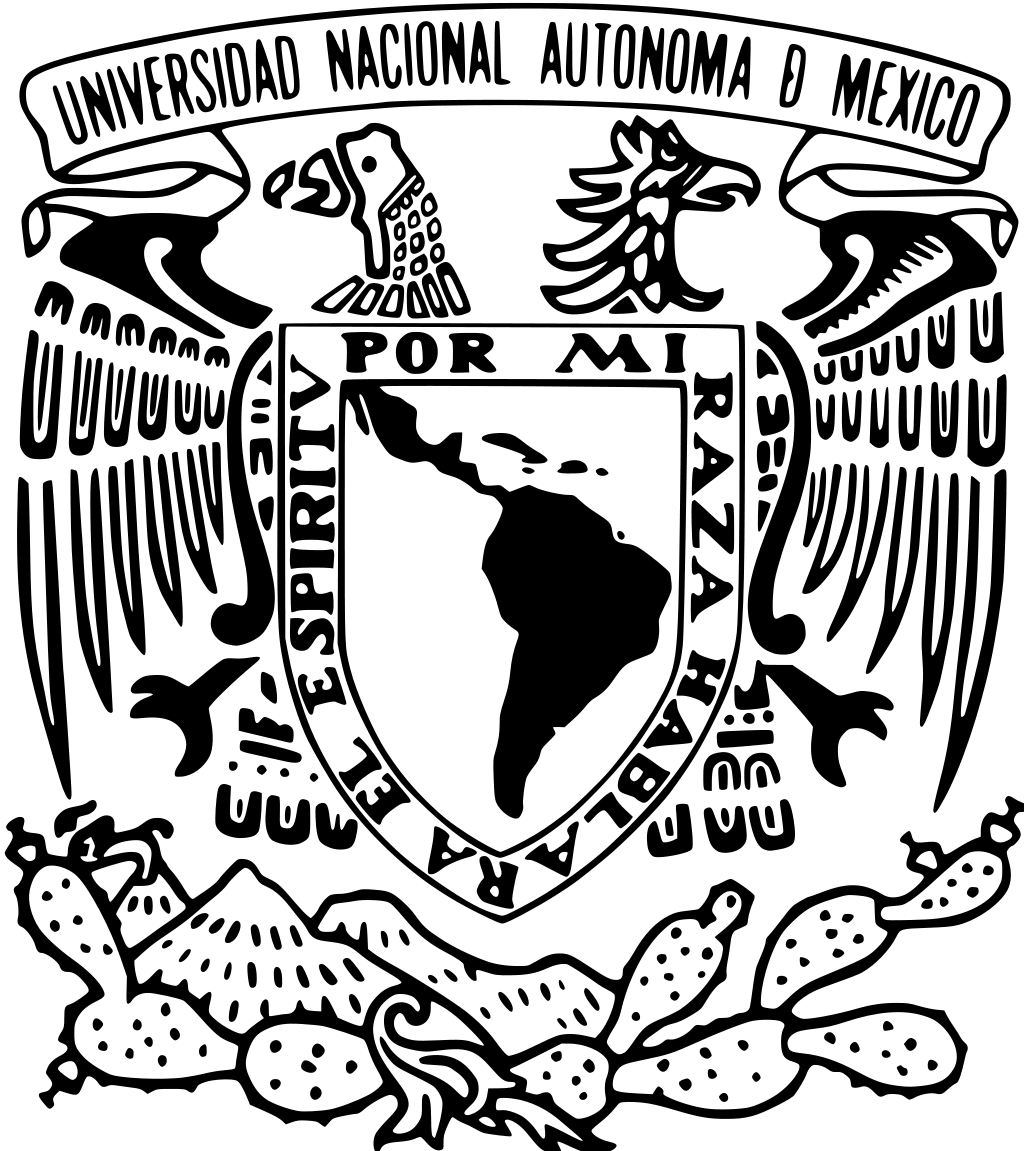
\includegraphics[width=0.3\textwidth]{unam_logo}\vfill{}
    {\scshape{\Huge Facultad de Ingeniería\par{}}}\vspace{0.5cm}
    {\scshape{\Large Sistemas Distribuidos\par{}}}\vfill{}
    {\huge \textbf{Proyecto}}\vfill{}

    {\Large
      Alumnos
      \begin{itemize}
        \item Gonzalez Gonzalez Claudio
        \item Mansur Jiménez Arturo
        \item Romero Andrade Cristian
        \item Romero Andrade Vicente
      \end{itemize}
      % \textbf{Equipo  }

    }\vfill{}
    {\large Profesor: ING.~Guadalupe Lizeth Parrales Romay}\vfill{}
    
\includegraphics[width=0.1\textwidth]{inge_logo}
  }
\end{titlepage}


\tableofcontents{}

% \lstlistoflistings{}
\clearpage{}

\section{Arquitectura}\label{sec:arq}
\begin{figure}[h!]
  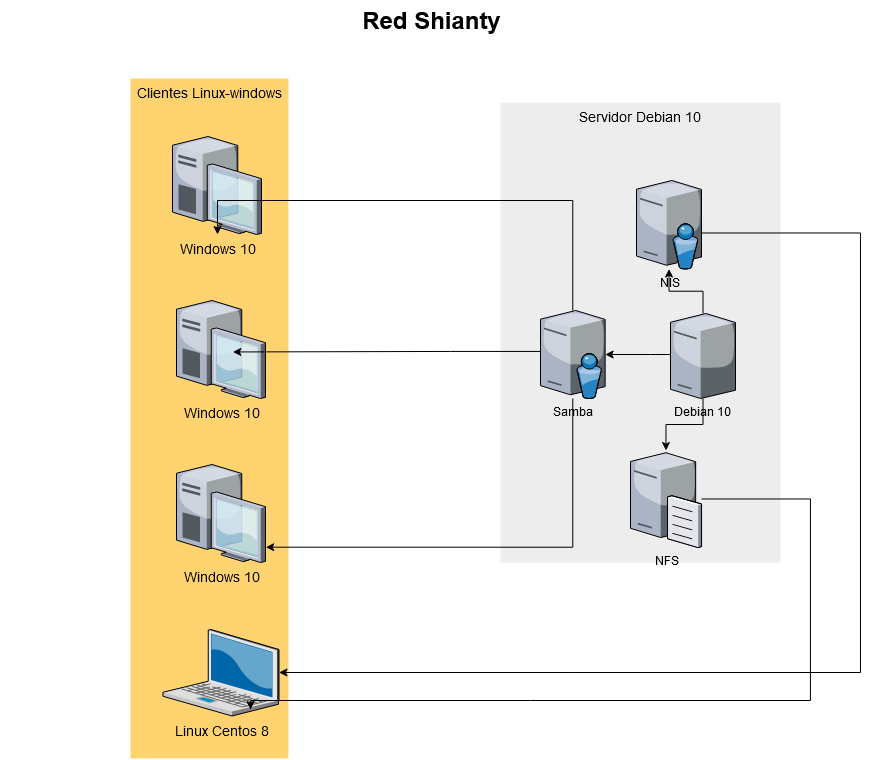
\includegraphics[width=0.9\textwidth]{arquitectura}
  \caption{Arquitectura de la red}\label{fig:arquitectura}
\end{figure}

\begin{figure}[h!]
  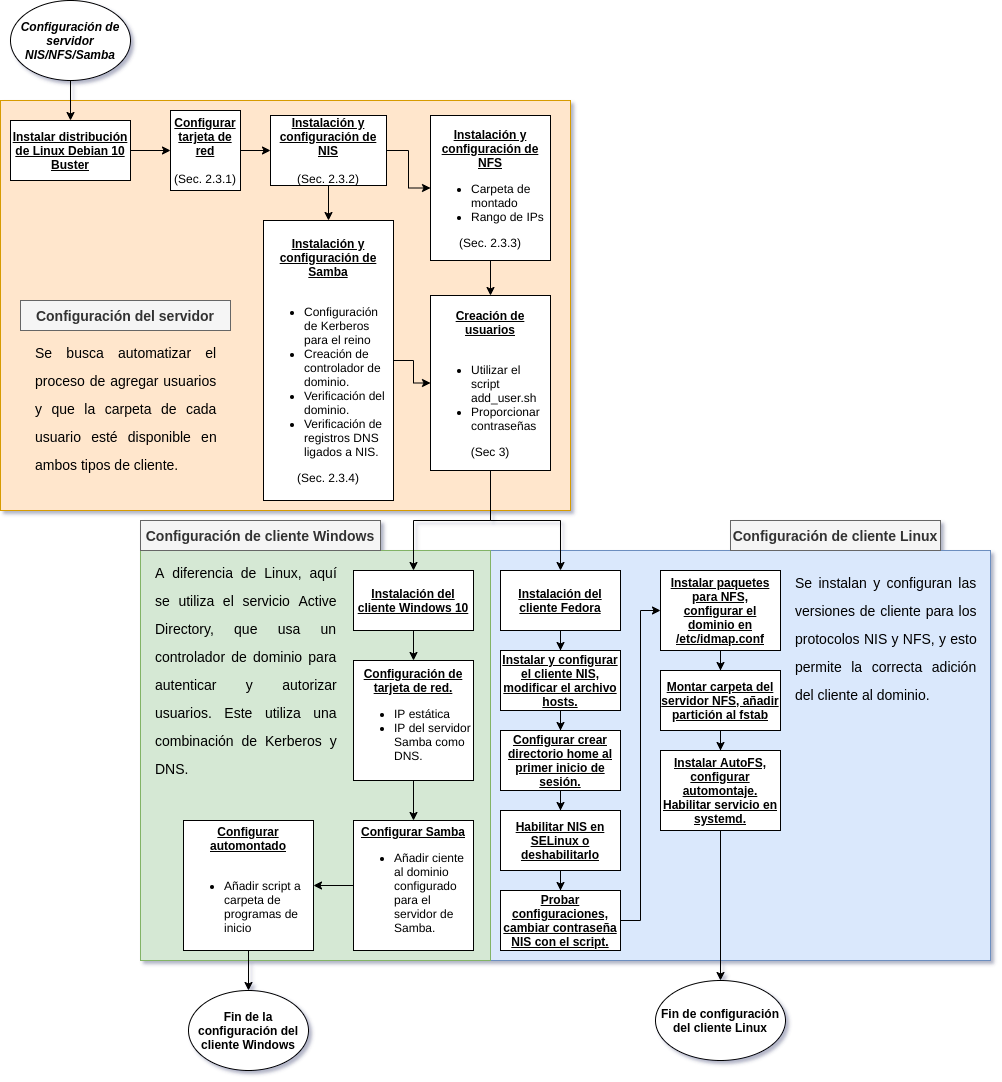
\includegraphics[width=0.9\textwidth]{Diagrama_Shianty}
  \caption{Diagrama cliente-servidor}\label{fig:dia_c_s}
\end{figure}



\section{Recursos}\label{sec:recursos}

\subfile{contenido/material_utilizado.tex}

\clearpage{}

\section{Creación de Usuarios}\label{sec:cusuarios}

\subfile{contenido/usuarios.tex}

\clearpage{}

\section{Clientes}\label{sec:clientes}

\subfile{contenido/cliente.tex}

\newpage

% \listoffigures\addcontentsline{toc}{section}{Índice de figuras}
% \listoflistings\@
% \addcontentsline{toc}{section}{Índice de códigos}


\end{document}
